% minipremessa
In questo capitolo iniziale forniremo una definizione di \textbf{DL} (Description Logics), analizzeremo le sue componenti e verranno descritte brevemente le sue estensioni più importanti, utilizzate negli ultimi anni.
\section{Informazioni iniziali}
Le logiche descrittive sono una famiglia di formalismi per la rappresentazione
della conoscenza, con la capacità di descrivere ciò che è noto in un dominio di
applicazione (detto mondo). Tale rappresentazione si fonda su strutture importanti,
come grafi o frames, e ha una difficoltà variabile, che dipende dal linguaggio scelto,
poiché l'espressività e la complessità computazionale sono direttamente proporzionali.
Tipicamente i nodi rappresentano concetti (oggetti), che possono
avere proprietà (semplici o articolate) associate. È piuttosto
semplice creare una corrispondenza tra i grafi e le \textbf{DL},
perché queste ultime sono dotate di predicati facilmente equiparabili alle strutture dei grafi:
\textit{predicati} unari corrispondo agli insiemi di individui, 
\textit{predicati} binari rappresentano relazioni tra singoli e infine un meccanismo di istruzioni 
d'inclusione per esprimere proprietà appartenenti ai concetti, come, ad esempio, \textit{Scimmia }$\sqsubseteq$\textit{ Mammifero}.

\begin{figure}[ht]
	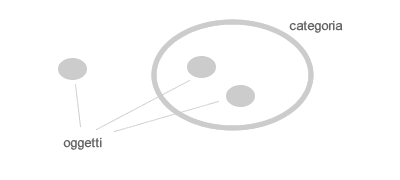
\includegraphics[width=\linewidth]{oggetti-categoria}
	\centering
	\caption{Un esempio di grafo}
\end{figure}

Ecco alcuni esempi riguardanti individui:
\begin{itemize}
	\item \textit{Volpe(foxy)}
	\item \textit{Scappa(foxy)}
	\item \textit{Gallina(coco)}
	\item \textit{Ruba(foxy,coco)}
	\item \textit{Uomo(jhon)}
	\item \textit{Insegue(jhon,foxy)}
\end{itemize}

È anche possibile utilizzare l’intersezione di concetti tramite la sintassi 
\textit{Cane} $\sqcap$ \textit{Taglia Grossa} per cercare individui che 
appartengono ad entrambe le categorie. \\
Ricordiamo che questa tipologia di logiche 
ha alla base quella del prim'ordine, da cui eredita la capacità di 
ragionamento attraverso inferenza, come il \textit{modus ponens}.
Infatti se all'insieme precedente aggiungessimo che:
\[\textit{Mammifero} \sqsubseteq \textit{Animale}\]
allora da questo potremo inferire che $\textit{Volpe}\sqsubseteq\textit{Animale}$.

Per queste e altre caratteristiche peculiari le DL sono ampiamente utilizzate in numerosi
sistemi, proprio per il buon compromesso tra capacità di rappresentazione,
ragionamento e complessità.\\
Vediamo, in breve, alcuni dei principali domini applicativi:

\paragraph{Data mining} 
Questo campo, da sempre al centro di molti dibattiti (anche etici),
ha come scopo "l'estrazione" di dati grezzi. Successivamente, al fine di classificarli,
viene fatto largo utilizzo delle logiche descrittive, per poi,
in seguito, attraverso tecniche di ragionamento, fare inferenza su 
di essi ed ottenere nuova conoscenza.

\paragraph{Medicina}
Fin dagli anni ’80 al centro di molte iniziative è stata la
creazione di una grande ontologia delle conoscenza medica, volta ad essere
di supporto nelle diagnosi. Per far fronte alla scalabilità della base di
conoscenza, si sono spesso utilizzate logiche descrittive basilari.
Rappresenta l'ambito di maggiore interesse per questo studio.

\paragraph{Configuration management}
È uno dei campi di maggior successo: esso include applicazioni che supportano
la progettazione di sistemi complessi grazie  all'unione di componenti multipli.
In particolare attraverso la classificazione di concetti (che possono
anche essere basate su modelli object oriented) si può creare una tassonomia che,
unita alla possibilità di ragionamento, intrinseca nelle logiche
descrittive, permette di trovare con facilità eventuali inconsistenze nel sistema.

\paragraph{Ingegneria del software}
Uno dei primi domini di applicazione: l’idea
alla base era di implementare, attraverso le logiche descrittive, un 
sistema che permettesse allo sviluppatore di trovare facilmente informazioni rilevanti
riguardo ad un sistema particolarmente grande e/o complesso.

\section{Caratteristiche e limiti}
\subsection{Tipologia ed Ingredienti}
% Da rivedere
Ogni logica descrittiva è caratterizzata da una particolare capacità espressiva che
varia a seconda delle possibilità e delle restrizioni imposte nei seguenti elementi:
\begin{itemize}
	\item $\mathcal{AL:}$ indica la logica degli attributi e introduce gli operatori 
	di congiunzione e quantificazione universale ed esistenziale;
	\item $\mathcal{C:}$ descrive la possibilità di usare l’operatore di negazione;
	\item $\mathcal{S:}$ indica la capacità di definire la chiusura transitiva di un ruolo;
	\item $\mathcal{H:}$ fornisce la potenzialità di definire gerarchie tra ruoli;
	\item $\mathcal{O:}$ asserisce la presenza dell'operatore di enumerazione;
	\item $\mathcal{I:}$ permette di riferirsi al ruolo inverso;
	\item $\mathcal{F}\ \mathcal{N}\text{ e }\mathcal{Q:}$ caratterizzano le disponibilità 
	di definire, rispettivamente, la cardinalità funzionale, semplice e qualificata (in ordine di espressività crescente);
	\item $\mathcal{D:}$ descrive la possibilità di riferirsi a domini concreti.
\end{itemize}
\subsection{Monotonicità}
Caratteristica peculiare delle \textbf{DL} nella forma di
\[ KB \models Q \implies KB \cup \{F\} \models Q\]
ovvero, se da una base di conoscenza \textbf{KB} si può concludere un fatto $ Q $, 
allora lo stesso fatto $ Q $ si deduce dalla stessa base di conoscenza arricchita con un nuovo fatto F.

Questa proprietà in sè è molto \textit{importante}, tuttavia non sempre si rivela pratica, anzi, 
esistono contesti (come il nostro) in cui, più che dare benefici, rende difficile il 
ragionamento e la deduzione di nuove informazioni.
Vediamone il perché con un famoso esempio.\\
Consideriamo la seguente base di conoscenza o \textit{Knowledge Base} tratta da \cite{PEAR}:     
\begin{itemize}
	\item[] \textit{Piove} $\implies$ \textit{Prendo(ombrello)}
	\item[] \textit{Piove}
\end{itemize}
si può banalmente concludere che: \textit{Prendo(ombrello)}

Aggiungiamo ora la seguente \textit{formula}
\begin{itemize}
	\item[] \textit{Sono\_Squattrinato}
\end{itemize}
La conclusione precedente rimane lecita anche dopo l'arricchimento della \textbf{KB}.

Aggiungiamo, invece, questa \textit{espressione}
\begin{itemize}
	\item[] \textit{Ho\_Perso(ombrello)}
\end{itemize}
Contro le nostre aspettative/intuizioni la conclusione non cambia, poiché dalle due premesse 
iniziali si giunge allo stessa conclusione senza che la nuova "conoscenza" influisca sul risultato.
Questo semplice modello ci mostra perché è importante, in contesti
specifici, avere dei linguaggi e degli automatismi in grado di tenere conto della 
realtà dei fatti, cioè una logica che possegga una \textbf{eredità rivedibile}.
\section{Il linguaggio base $\mathcal{AL}$}
Un sistema di rappresentazione della conoscenza basato sulle \textbf{DL}
permette di creare, manipolarle e ragionare su diverse \textit{Knowledge Base}.\\
Ma cos'è formalmente una \textbf{KB}?
La base di conoscenza è composta principalmente da una coppia \textit{(T,A)} 
$\mathrm{TBox} \text{ e } \mathrm{ABox}$.
La prima introduce i concetti, insiemi di individui, e ruoli, che
denotano relazioni binarie tra i concetti. \\
Invece per quanto concerne la seconda, essa contiene asserzioni su singoli individui, riguardanti 
concetti della $\mathrm{TBox}$.
Definiamo come descrizioni elementari i concetti e ruoli atomici. Invece trattiamo come 
complesse le descrizioni che possono essere costruite attraverso induzione.
In notazione useremo le lettere $A$ e $B$ per indicare
concetti atomici, la lettera $R$ per rappresentare i ruoli atomici e le lettere $C$ e
$D$ per le descrizioni dei concetti. Qui sotto daremo una definizione di $\mathcal{AL}$ \cite{DLHandbook},
linguaggio minimo di interesse pratico, su cui si basano tutti gli altri linguaggi di questa famiglia.

Le descrizioni di concetti sono definite secondo le seguenti regole sintattiche:
\begin{itemize}
	\item[] \makebox[2cm]{$C,D \to$\hfill}
	\item[] \makebox[2cm]{$\top$ \hfill} (concetto atomico)
	\item[] \makebox[2cm]{$\bot$ \hfill} (top concept - generico)
	\item[] \makebox[2cm]{$\neg\ A$ \hfill} (negazione atomica)
	\item[] \makebox[2cm]{$ C \sqcap D$ \hfill} (intersezione)
	\item[] \makebox[2cm]{$\forall R.C $ \hfill} (restrizione di valore)
	\item[] \makebox[2cm]{$\exists R. \bot$ \hfill} (quantificazione esistenziale limitata)
\end{itemize}
Per definire una semantica formale per i concetti di $\mathcal{AL}$ poniamo alla base 
l'idea di modello e l'idea di funzione d'interpretazione:
\begin{equation} \label{model}
\mathcal{M} = \langle \Delta;fx \rangle
\end{equation} 
\begin{equation} \label{fun}
fx: A \to \Delta
\end{equation}
Definito che le interpretazioni $\mathcal{I}$ sono sottoinsiemi non vuoti di $\Delta$ (dominio dell'interpretazione),
lo scopo di \ref{model} è quello di fornire un significato alle formule, mentre, 
per quanto riguarda \ref{fun}, quello di
permettere di assegnare a ogni concetto atomico $\mathit{A}$ un insieme 
$\mathit{A^{\mathcal{I}} \subseteq \Delta^{\mathcal{I}}}$ 
e per ogni ruolo atomico $\mathit{R}$ una relazione binaria 
$\mathit{R^{\mathcal{I}} \subseteq \Delta^{\mathcal{I}} \times \Delta^{\mathcal{I}}}$.\\
La funzione di interpretazione è estesa alla descrizione di concetti attraverso le seguenti definizioni induttive :
\begin{itemize}
	\item[] \makebox[2cm]{$\top^{\mathcal{I}}$\hfill} = $\Delta^{\mathcal{I}}$  
	\item[] \makebox[2cm]{$(\neg A)^{\mathcal{I}}$ \hfill} = 
	$\Delta^{\mathcal{I}}\backslash A^{\mathcal{I}}$
	\item[] \makebox[2cm]{$(C \sqcap D)^{\mathcal{I}} $ \hfill} = 
	$ C^{\mathcal{I}} \sqcap D^{\mathcal{I}} $  
	\item[] \makebox[2cm]{$(\forall R.C)^{\mathcal{I}}$ \hfill} = 
	$\{x \in \Delta| \forall y.(x,y) \in R^{\mathcal{I}} \to y \in C^{\mathcal{I}} \}$
	\item[] \makebox[2cm]{$(\exists R.\top)^{\mathcal{I}}$ \hfill} = 
	$\{x \in \Delta| \exists y.(x,y) \in R^{\mathcal{I}} \}$
\end{itemize}
Diciamo che due concetti $C, D$ sono equivalenti, e scriviamo $C = D$, se
$C^{\mathcal{I}} = D^{\mathcal{I}}$ per ogni interpretazione ${\mathcal{I}}$.
\paragraph{Aggiunta di $\mathcal{C}$: l’operatore di negazione} \hfill \\
A questo linguaggio, possiamo aggiungere l’estensione di negazione, un concetto arbitrario:
\begin{itemize}
	\item[] \makebox[4cm]{$ \neg C $ } (concept negation)
\end{itemize}
La cui semantica risulta essere:
\[ (\neg C)^{\mathcal{I}} =  \Delta^{\mathcal{I}}\backslash C^{\mathcal{I}}\]
Grazie a questa aggiunta il linguaggio $ \mathcal{AL} $ si arricchisce, 
passando ad essere la logica descrittiva $ \mathcal{ALC} $.
\paragraph{Esempio} \hfill
\\
Vediamo un semplice caso che faccia uso di questa nuova sintassi 
\textit{ABox}
\begin{itemize}
	\item $ Volpe(foxy)$
	\item $ Gallina(coco) $
	\item $ Uomo(jhon) $
\end{itemize}
\textit{TBox}
\begin{itemize}
	\item $ \forall x,y |(Volpe(x) \land \textit{Affamata}(x)) \land Gallina(y)  \implies Ruba(x,y) $
	\item $ \exists x,y |Uomo(x) \land Gallina(y) \land Ama(x,y) \implies \neg Uccide(x,y) \land Protegge(x,y) $
\end{itemize}
Per ogni volpe e gallina, se la \textit{Vulpes} è affamata allora ruba il \textit{Gallus domesticus}
Di conseguenza se esiste una gallina e un uomo che la ama, questo non la ucciderà ma la proteggerà (dalla volpe).

\clearpage

\section{Operatore T}
\subsection{Premessa}
L'obbiettivo della \textit{TBox} è costruire una tassonomia di concetti (\textit{ossia} un albero di classificazione). 
Come rappresentare le proprietà dei prototipi e ragionare sulla loro perdita a livelli inferiori? \\
Data una tassonomia $T$, con $A$ e $B$ tali che $A$ è un concetto “padre“ di $B$, 
non sempre tutte le proprietà di $A$ possono essere ereditate da $B$.\\
L’approccio tradizionale a questo problema è di gestire le perdite di proprietà 
integrando alcuni meccanismi di ragionamento non monotono, portando allo studio di estensioni 
delle logiche descrittive in questo ambito e cercando di superare il limite.
\subsection{Definizione di T}
Idealmente un'estensione possibile dovrebbe possedere almeno le seguenti caratteristiche:
\begin{enumerate}
	\item una chiara semantica, basata sulla stessa della logica sottostante;
	\item la possibilità di specificare proprietà dei prototipi in maniera naturale e diretta;
	\item mantenere la decidibilità (già ereditata) e dimostrabile attraverso il metodo convenzionale.
\end{enumerate}
Vediamo dunque come nel lavori \cite{DLExtension} e \cite{COCOS} si faccia uso dell'operatore $ \mathbf{T} $ di 
tipicalità per l'inferenze. La nostra \textbf{KB} ha, in aggiunta, un insieme di asserzioni della forma
$ \mathbf{T}(C) \sqsubseteq D $ o $ \mathbf{T}(C)(m) $ dove $ D $ è un concetto che non menziona $ C $.

Supponiamo che la \textit{Tbox} contenga:
\begin{itemize}
	\item[] $ T(Student) \sqsubseteq \neg IncomeTaxPayer$
	\item[] $ T(Student \sqcap Worker) \sqsubseteq IncomeTaxPayer$
	\item[] $ T(Student \sqcap Worker \sqcap Erasmus) \sqsubseteq \neg IncomeTaxPayer $
\end{itemize}
Interpretando \textbf{T} come "tipico/i", questa corrisponde alle asserzioni:
\begin{itemize}
	\item[] (I $T$ studenti non sono tassati)
	\item[] (I $T$ studenti-lavoratori sono tassati)
	\item[] (I $T$ studenti-lavoratori in erasmus non sono tassati)
\end{itemize}
Ipotizziamo che la \textit{ABox} contenga, in alternativa, uno dei seguenti fatti:
\begin{enumerate}
	\item $ Student(andrea) $
	\item $ Student(agnese), Worker(agnese) $
	\item $ Student(damiano), Worker(damiano), Erasmus(damiano) $
\end{enumerate}
Dunque possiamo inferire le aspettate conclusioni:
\begin{enumerate}
	\item $ \neg IncomeTaxPayer(andrea) $
	\item $ IncomeTaxPayer(agnese) $
	\item $ \neg IncomeTaxPayer(damiano) $
\end{enumerate}
Se \textit{ABox} contenesse l'espressione $ \exists HasBrother.Student(davide) $ è possibile dedurre
proprietà di individui implicitamente introdotte dalla restrizione esistenziale, come:
\[ \exists HasBrother.\neg IncomeTaxPayer(davide) \]
Infine, aggiungere informazioni irrilevanti non dovrebbe modificare le conclusioni.
Ammettendo, infatti, che la \textit{TBox} precedente abbia la seguente forma:
\begin{itemize}
	\item[] $ T(Student \sqcap Short) \sqsubseteq \neg IncomeTaxPayer$
	\item[] $ T(Student \sqcap Worker \sqcap Short) \sqsubseteq IncomeTaxPayer$
	\item[] $ T(Student \sqcap Worker \sqcap Erasmus \sqcap Short) \sqsubseteq \neg IncomeTaxPayer $
\end{itemize}
possiamo concludere che \textit{Short} è un’informazione irrilevante rispetto all'essere tassati.
Per la stessa ragione, la conclusione che Andrea sia un’istanza di\\
$ \neg IncomeTaxPayer(andrea)$ o meno, non è influenzata qualora si aggiunga l'espressione
$ Tall(andrea) $ alla \textit{ABox}.
\clearpage

\section{La logica $ \mathcal{ALC} + \mathbf{T} $}
Dato un alfabeto contenti nomi di Concetti $ \mathcal{C} $, di Ruoli $ \mathcal{R} $ e costanti di
individui $ \mathcal{O} $ il linguaggio $ \mathcal{L} $ appartenente alla logica $ \mathcal{ALC} + \mathbf{T} $
viene definito a partire dalla distinzione chiave tra \textit{Concetti} e \textit{Concetti Estesi} \cite{DLExtension}
\begin{multicols}{2}
	\begin{itemize}
		\item[] $ Concetti $
		\item[] \begin{itemize}
			\item[] $ A \in \mathcal{C}, \top \text{ e } \bot $ sono \textit{concetti} di $ \mathcal{L} $
			\item[] se $ C,D \in \mathcal{L} \text{ e } R \in \mathcal{R} $ allora
			 $ C \sqcap D,C \sqcup D \neg C, \forall R.C, \exists R.C $ sono concetti di $ \mathcal{L} $
		\end{itemize}
	\end{itemize}
	\begin{itemize}
		\item[] $ Concetti Estesi $
		\item[] \begin{itemize}
			\item[] se $ C $ è un \emph{concetto} di $ \mathcal{L} $, allora $ C $ e $\mathbf{T}(C)$ 
			sono \textit{concetti estesi} di $ \mathcal{L} $
			\item[] combinazioni booleane di concetti estesi sono a loro volta \textit{concetti estesi} di $ \mathcal{L} $.
		\end{itemize}
	\end{itemize}
\end{multicols}
La base di conoscenza \textbf{KB} conserva la coppia \textit{(Tbox, Abox)} dove:
\begin{itemize}
	\item $ Tbox $: contiene asserzioni $ C \sqsubseteq D \text{, dove } C \in \mathcal{L} $ è un 
	\textit{concetto esteso} della forma $ C'$ oppure $ \mathbf{T}(C') $, mentre $ D \in \mathcal{L} $ è un \textit{concetto}
	\item $ Abox $: composta da espressioni $ C(a) $ e $ aRb $ dove $ C \in \mathcal{L} $ è un 
	\textit{concetto esteso}, $ R \in \mathcal{L} $ e $ \mathcal{O} $
\end{itemize}
Estendiamo la definizione di Modello utilizzato nella terminologia logica sottostante, 
al fine di fornire una semantica all'operatore $ \mathbf{T} $
\[ \mathcal{M} = \langle \Delta;I;< \rangle\]
$ \Delta $ è il domino. $ I $ è la funzione di estensione.
Ecco il nuovo elemento, una relazione d'ordine, non riflessiva, transitiva e modulare, che ha la funzione di determinare, all'interno della \textit{Knowledge Base}, quali individui siano tipici e quali no.
\begin{figure}[h]
	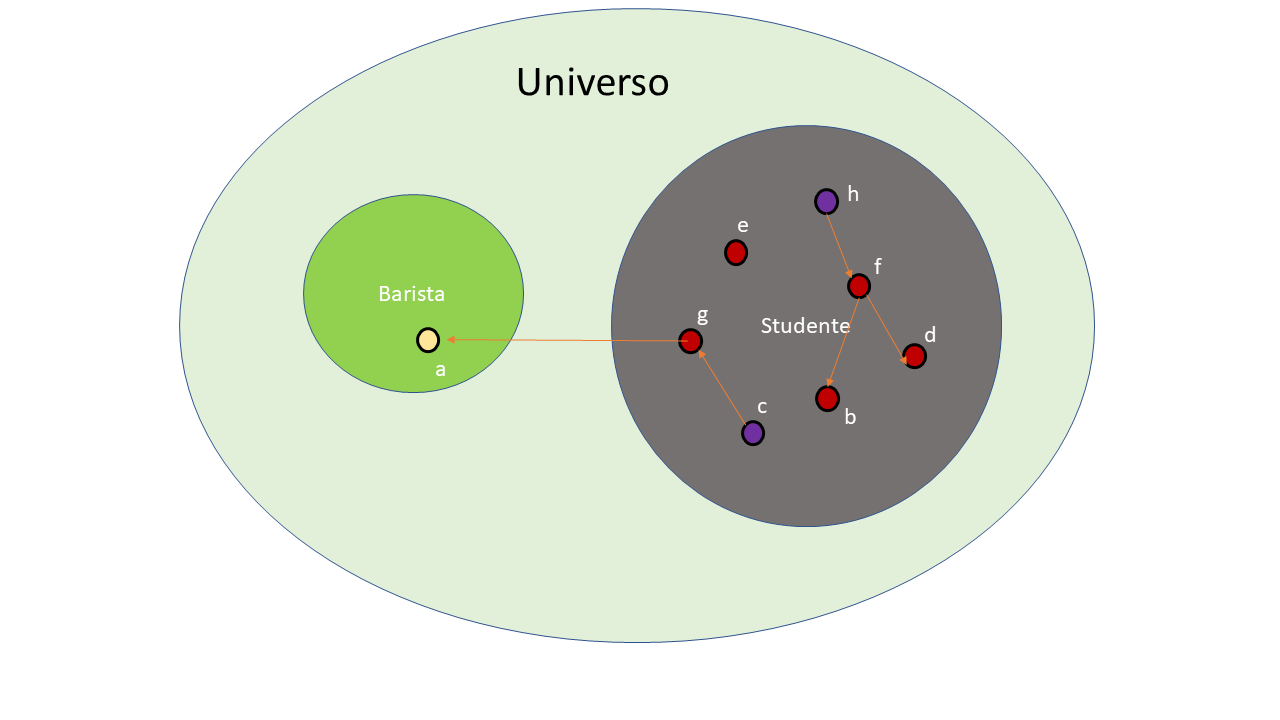
\includegraphics[width=\textwidth]{FdiValutazione.png}
	\label{fig:valutaz}
	\centering
\end{figure}
\clearpage
Intuitivamente un individuo \textit{m} è \textbf{tipico} se non esiste alcun elemento più \textit{normale},
viceversa, un  \textit{n} è \textbf{atipico} quando esiste almeno un individuo più \textit{normale}.
Indichiamo formalmente che l'espressione:
\begin{itemize}
	\item[] \makebox[4cm]{$ x < y $} (l'individuo $ x $ è più \textit{normale} di $ y $)
\end{itemize}
Consideriamo dunque l'esempio \ref{fig:valutaz} della pagina precedente:\\
gli studenti tipici sono $ b,c,d,e,f,g,h $, in particolare, $ e $ è tipico perché non è in alcuna
relazione del tipo $ x < y $, per quanto riguarda la catena$  h, f, d, b $ si evince che $ d $ e $ b $ siano più
\textit{normali} di $ f $ che a sua volta è più \textit{normale} di $ h $;\\ 
come conseguenza $ d $ e $ b $ risultano essere tipici poiché questa catena non prosegue bensì termina con loro due. 
Invece non risulta corretto concludere che $ g $ sia uno studente tipico, infatti, nonostante sia 
più normale di $ c $, è in relazione con $ a $, tuttavia $ a $ appartiene 
ad un insieme diverso (Barista) e questo non influisce sulla sua "tipicità".
La relazione di preferenza ha limite di essere parziale, 
infatti non è sempre possibile stabilire quale elemento sia più tipico degli altri.

In realtà l’estensione di questa sezione viene chiamata $ \mathcal{ALC + \mathbf{T_{R}}} $ dove il pedice
R indica il concetto di logica razionale sulle cui proprietà si basa la semantica di
T. Tali caratteristiche, come la \textit{specificità}, costituiscono le fondamenta del ragionamento non monotono, 
permettendo modellare la situazione in questo modo:

\begin{figure}[h]
	\caption{Un esempio di modello}
	\label{fig:esempioM}
	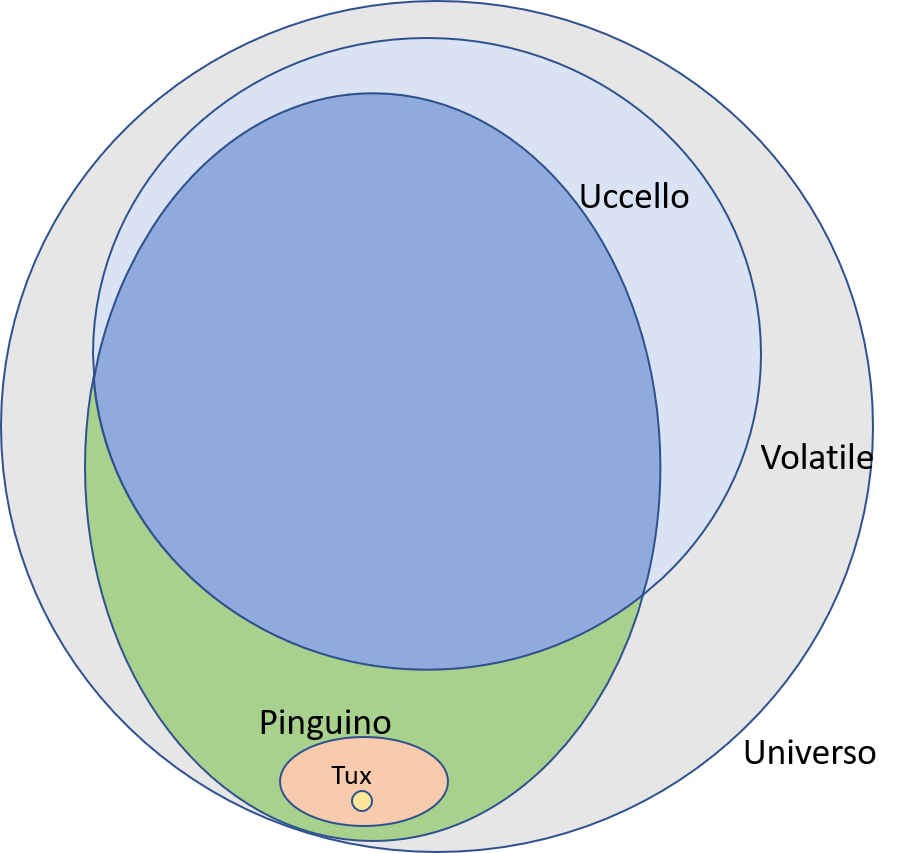
\includegraphics[height=13cm,width=\textwidth]{immagini/ModelloALC_T.png}
	\centering
\end{figure}
Nella Figura \ref{fig:esempioM} è possibile rappresentare Tux (un \textit{Pinguino}) come è un uccello che non vola;
graficamente quest'informazione è racchiusa nella zona verde dell'insieme Uccello,
ovvero, quella sezione popolata da tutti gli uccelli atipici, mentre la porzione in blu rappresenta gli elementi tipici.

\section{La logica non monotona $ \mathcal{ALC} + \mathbf{T}_{\mathbf{R}}^{\mathit{RaCl}} $}
Nonostante l'aggiunta dell'operatore $ \mathbf{T} $ la logica appena vista rimane monotona, 
nel senso che se il fatto $ F $ segue da una certa base
di conoscenza \textbf{KB} , allora lo stesso fatto $ F $ segue da una qualsiasi $ KB' \subseteq KB $. 
Di conseguenza, a meno che una base di conoscenza contenga delle assunzioni esplicite circa la tipicalità degli individui, non esiste alcun modo per inferire proprietà rivedibili su di loro. \\
Un'altra limite riguarda l'intrattabilità della \textit{irrilevanza}.
\begin{itemize}
	\item[] $ LottatoreDiSumo \sqsubseteq Atleta $
	\item[] $ \mathbf{T}(Atleta) \sqsubseteq \neg Grasso $
	\item[] $ \mathbf{T}(LottatoreDiSumo) \sqsubseteq Grasso $
\end{itemize}
per via della monotonia di $ \mathcal{ALC + \mathbf{T_{R}}} $ non si può derivare che:
\[ \mathbf{T}(LottatoreDiSumo \sqcap Orientale) \sqsubseteq Grasso \] 
malgrado l'etnia sia totalmente irrilevante rispetto all'essere grassi o magri.

Con l'obbiettivo di creare inferenze non monotone utili gli autori in \cite{FromPLtoDL} hanno rinforzato la semantica precedente restringendo le assegnazioni ad una classe minimale di modelli. 
L’idea è quella di restringere l’assegnazione a modelli minimi che \textit{minimizzino l'atipicalità dei concetti} e
dove le inclusioni implicate sono quelle che appartengono alla chiusura razionale della base di conoscenza, 
estensione naturale di \cite{Conditional_KB}.

Considerare solo i modelli che massimizzano le istanze tipiche di un concetto quando sono 
consistenti con la base di conoscenza.
Senza entrare troppo nei dettagli la semantica $\mathcal{ALC} + \mathbf{T}_{\mathbf{R}}^{\mathit{RaCl}}$
non monotona si basa su modelli razionali minimi che riducono al minimo il \textit{rank} degli elementi del dominio.

Intuitivamente, dati due modelli $ \mathcal{M_1,M_2} $ di una \textbf{KB} se è noto che 
in $ M_1 $ un elemento $ x $ ha rank 2 (a causa di istanze $ z < y < x $) ed
in $ M_2 $ $ x $ ha rank 1 (a causa di $ y < x $), noi preferiamo il secondo,
perché l’elemento x risulta più tipico che in $ M_1 $.
I modelli vengono quindi selezionati per il ragionamento scartando quelli grado più elevato poiché in essi gli elementi sono meno "tipici" e quindi verrebbero dedotte meno informazioni (vedi anche Figura a pagina \pageref{fig:valutaz}).

\clearpage

\subsection{Traduzione dell'operatore T} \label{subSec: Traduzione T}
In alcuni contesti non è sempre possibile modificare l'intera struttura basata su logiche consolidate.
È sensato chiedersi quale sia il significato di questo operatore e se esistano formulazioni equivalenti.
Consideriamo la \textit{TBox}:
\[ \mathbf{T}(Pesce) \sqsubseteq Oviparo \]
Come sappiamo esprime il fatto che, tipicamente, gli uccelli sono ovipari (depositano le uova). \\
Ecco la traduzione equipollente, vista in \cite{PEAR} e \cite{COCOS}, senza far uso dell'operatore $ \mathbf{T} $ è la seguente: 
\begin{enumerate}\label{enu:elencoCond}
	\item $ Pesce \sqcap Pesce1 \sqsubseteq Oviparo $
	\item $ Pesce1 \sqsubseteq \forall R(\neg Pesce \sqcap Pesce1) $
	\item $ \neg Pesce1 \sqsubseteq \exists R(Pesce \sqcap Pesce1) $
\end{enumerate} 
Questa traduzione implementa la relazione d'ordine $ < $ precedentemente introdotta.\\
L'insieme $ Pesce1 $ rappresenta i pesci tipici mentre $ Pesce $ contiene tutti i possibili pesci, 
compresi quelli atipici, e costituisce infatti un soprainsieme di Pesce1. \\ 
La suddivisione in questi due insiemi a \ref{fig:tradPesce} è fondamentale per poter tenere traccia delle eccezioni, ottenendo così la possibilità di ragionare sia sull'individuo generico sia sul tipico individuo.\\
\begin{figure}[h]
	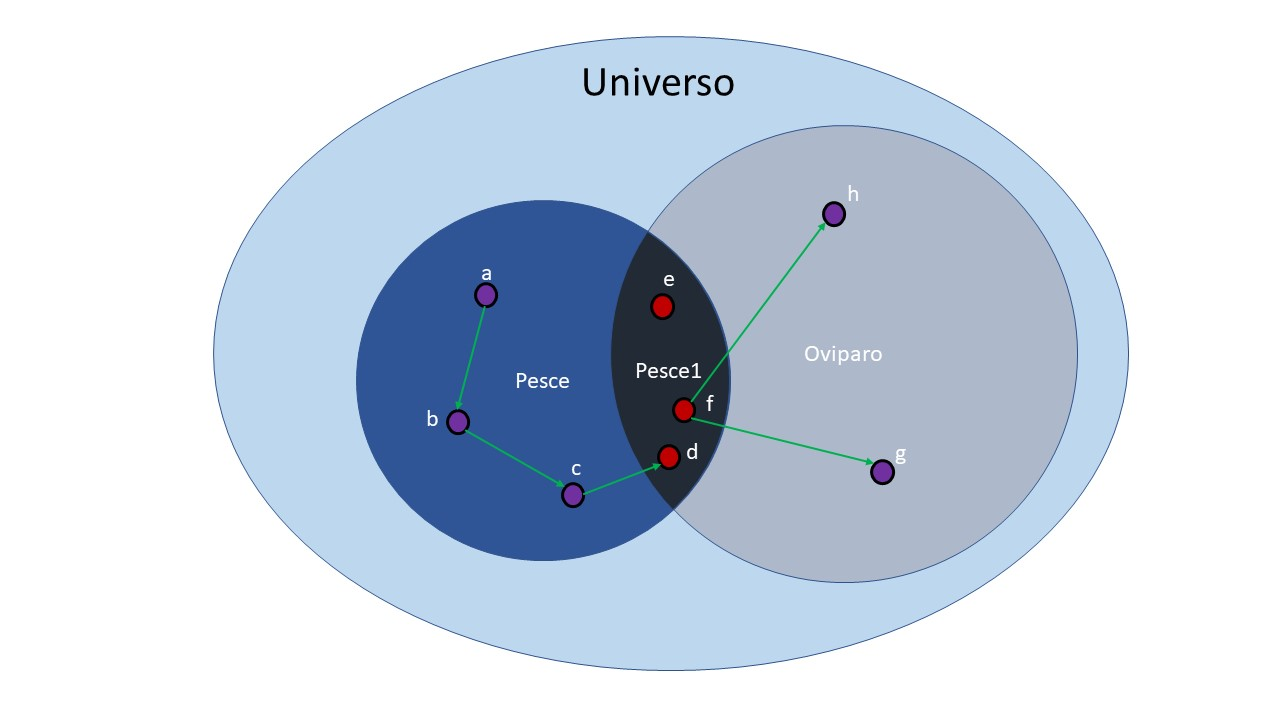
\includegraphics[width=\textwidth]{Traduzione_T_.jpg}
	\centering
	\caption{Esempio traduzione $ \mathbf{T}(Pesce) \sqsubseteq Oviparo $}
	\label{fig:tradPesce}
\end{figure}
Pertanto per inferire che $ nemo $ sia un tipico $ Pesce $ controllerà che la seguente espressione sia vera:
\[ \mathbf{T}(Pesce)(nemo) \iff Pesce(nemo) \land Pesce1(nemo) \]

In caso di risposta affermativa sarà verificato che: 
\[ Pesce(nemo) \sqcap Pesce1(nemo) \sqsubseteq Oviparo(nemo) \]

Ecco quindi verificata la condizione $ 1 $ di \ref{enu:elencoCond}
Viceversa la definizione $ 2 \text{ e } 3 $ esprimono formalmente cosa significhi essere un individuo a/tipico.
\begin{multicols}{2}
	$ Pesce1 \sqsubseteq \forall R.(\neg Pesce \sqcap Pesce1) $ \\
	$ \neg Pesce1 \sqsubseteq \exists R.(Pesce \sqcap Pesce1) $
\end{multicols}
Nell'esempio \ref{enu:elencoCond}, i membri $ d,e \text{ ed } f $ sono pesci tipici. È evidente che l'intersezione
$ \neg Pesce \sqcap Pesce1 $ sia vuota. Dunque deduciamo che, dato l'insieme $ A $, se un elemento $ m \in A$ 
è \textbf{tipico} o non è in alcuna relazione del tipo $ x < y $ ()e quindi non esiste un 
individuo più normale di lui) o è più ordinario di un generico $ x $ $(m < x)$ con $ x \in A $ 
oppure si trovi nella relazione $ x < m $ dove però $ x \notin A $.

Per quanto concerne i pesci \textbf{atipici}, come le istanze $ a,b \text{ e } c $, per verificarne la tipicità 
viene svolto un procedimento molto simile. Prendiamo in esempio $ b $: viene verificato inizialmente lo stato
dell'elemento (se si trovi o meno in una o più relazioni) e analizzato. In questo caso scopriamo che è più 
caratteristico di $ a $ ma meno di $ c $ che, a sua volta, è più generico di $ d $, che scopriamo essere tipico.
Per transitività troviamo la relazione $ d < b $ che conferma a b la sua atipicità.
In conclusione, un membro è atipico quando esiste \textbf{almeno un} individuo più normale di lui

\section{La logica $ \mathcal{ALC} + \mathbf{T}_{\mathbf{R}}^{\mathtt{P}} $}
Dopo aver illustrato la logica di base $ \mathcal{ALC} $ ed introdotto l’estensione non monotona
$ \mathcal{ALC} + \mathbf{T} $ con i relativi concetti di \textbf{chiusura e logica razionale}, in questa sezione
verrà descritta l’estensione "accennata" nel capitolo introduttivo \ref{itemize: 3 comp} che permette di tenere in considerazione la probabilità di individui particolari \cite{ProbOfEx}.

\subsection{Modifiche alla semantica }
L'inclusione di tipicalità si evolve e va ad assumere la forma:
\[ \mathbf{T}(C) \sqsubseteq_{p} D \]
con il significato intuitivo aggiuntivo: la probabilità di avere un $ C $ eccezionale (cioè \textbf{atipico})
che non sia anche un $ D $ vale $ 1-p $.

La base di conoscenza (\textbf{KB}) $ (TBox,ABox) $ ha la seguente struttura
\begin{multicols}{2}
	$ TBox $ in cui $ p \in \mathbb{} e p \in (0,1) $
	\begin{itemize}
		\item $ C \sqsubseteq_{p} P $
		\item $ \mathbf{T}(C) \sqsubseteq_{p} P $
	\end{itemize} 
	$ ABox $ in cui $ a,b \in \mathcal{0} $
	\begin{itemize}
		\item $ C(a) $
		\item $ R(a,b) $
	\end{itemize}
\end{multicols}

È facilmente intuibile che più la probabilità p è alta più l’inclusione è "libera da eccezioni" o, 
equivalentemente, è meno probabile avere un C speciale che non è anche un D.\\
A tal proposito è importante sottolineare che la probabilità $ p $  con $ p = 1 $ non è consentita 
in quanto l’inclusione $ \mathbf{T}(C) \sqsubseteq_{1} D  $
corrisponde all'inclusione stretta $ \mathbf{T}(C) \sqsubseteq D $ che esprime invece il fatto che
l’elemento $ C $ è sicuramente anche un $ D $.\\
Data una seconda inclusione $ \mathbf{T}(C') \sqsubseteq_{p'} D' $, con $ p' < p $, si assume che questa
inclusione sia meno "restrittiva" rispetto alla prima in quanto la possibilità di avere un
eccezionale $ C' $ è più alta rispetto alla probabilità di avere un eccezionale $ C $, tenendo rispettivamente
conto delle proprietà $ D' \text{ e } D $.

Considerando, per esempio, la seguente \textit{TBox}
\begin{itemize}
	\item $ \mathbf{T}(Liceale) \sqsubseteq_{0.80} Studioso $
	\item $ \mathbf{T}(Liceale) \sqsubseteq_{0.60} PraticaDelloSport $
\end{itemize}
si evince che il tipico scolare è studioso e che, normalmente, pratica dello sport;
entrambe sono proprietà del prototipo dello studente, tuttavia ci sono più
eccezioni di studenti che non fanno sport rispetto a quelli che non studiano.

Una cosa importante da tenere in considerazione è la possibilità di avere \textit{Knowledge Base}
contenenti inclusioni con $ p \leq 0.5 $, che se
erroneamente interpretate, potrebbero venir considerate contro-intuitive.

Ad esempio,l’inclusione $ \mathbf{T}(Liceale) \sqsubseteq_{0.22} Fumatore  $  potrebbe venir erroneamente 
interpretata come "normalmente, gli studenti non sono fumatori"; anche se la corrispondente probabilità è bassa, 
la spiegazione corretta è che fare uso di sigarette è in ogni caso una 
proprietà del prototipo dello studente liceale.\\
A differenza dell'espressione $ \mathbf{T}(Liceale) \sqsubseteq_{0.80} Studioso $, si ha che la
probabilità di trovare studenti eccezionali non fumatori è più alta rispetto a quella
di trovare studenti eccezionali che siano studiosi.\\
%ma entrambe sono tipiche proprietà di uno studente.
Ponendo il caso in cui si volesse formalizzare che il tipico studente non è una persona giovane, bisogna 
semplicemente formulare l’inclusione $ \mathbf{T}(Liceale) \sqsubseteq_{0.78} \neg Fumatore  $ nella base di conoscenza.

\subsection{Estensione dell'\textit{Abox}}
Data una base di conoscenza \textbf{KB }, viene definito l’insieme finito $ \mathfrak{Tip} $ dei concetti che
occorrono all'interno dell'operatore di tipicalità, formalmente
\[ \mathfrak{Tip} = \{ C | \mathbf{T}(C) \sqsubseteq_{p} D \in KB \}. \]
Dato un individuo $ a $ esplicitamente dichiarato nell'\textit{ABox}, si definisce l’insieme delle
assunzioni di tipicalità $ \mathbf{T}(C)(a) $ che possono essere dedotte in maniera minimale dalla \textbf{KB}
nella logica non monotona $ \mathcal{ALC} + \mathbf{T}_{\mathbf{R}}^{\mathit{RaCl}} $, con $C \in \mathfrak{Tip}$.

Quindi si considera un insieme ordinato $ \mathfrak{Tip}_{\mathcal{A}}$ (dove $ \mathcal{A} $ sta per \textit{ABox})
di coppie $ (a, C) $ di tutte le possibili assunzioni $ \mathbf{T}(C)(a) $, 
per tutti i concetti $ C \in \mathfrak{Tip} $ e per tutti gli individui $ a $ nell'\textit{ABox}.

In aggiunta si definisce il multi-insieme ordinato $ \mathcal{P_{A}}$ tupla della forma $[p_1,p_2,...,p_n] $
dove $ p_i $ è la probabilità dell'assunzione $ \mathbf{T}(C)(a) $ tale che $ (a,C) \in 
\mathfrak{Tip}_{\mathcal{A}} $ alla posizione $ i $; inoltre rappresenta il prodotto di tutte le probabilità 
$ p_ij $ delle inclusioni $ \mathbf{T}(C) \sqsubseteq_{p_ij} D $ nella \textit{TBox}.

%Da rivedere wide tilde
Seguendo le idee di \cite{ReasoningOnScen}, si considerano diverse estensioni $ \mathcal{\widetilde{A}}_i $
dell'\textit{ABox} che vengono equipaggiate con una probabilità $ p_i $. Partendo dagli insiemi  
$ \mathcal{P_{A}} = [p_1,p_2,...,p_n] $ e $ \mathfrak{Tip}_{\mathcal{A}}$, il primo passo è quello 
di definire l'insieme $ \mathbb{S} $ di tutte le stringhe di possibili assunzioni, utilizzando lo 0 come $ p_i $ per rappresentare che la corrispondente asserzione di tipicalità non viene più assunta.

Successivamente, si definisce l’estensione $ \mathcal{\widetilde{A}}_i $ di $ \mathcal{{A}} $ 
corrispondente ad una stringa $ [s_1,s_2,...,s_n] \in \mathbb{S} $ cosi ottenuta. 
In questo modo, la probabilità più alta viene assegnata all'estensione dell'\textit{ABox} corrispondente a 
$ \mathcal{P_{A}} $, dove tutte le assunzioni di tipicalità vengono considerate.
mentre diminuisce nelle altre estensioni, alcune assunzioni di tipicalità vengono scartate, 
così 0 viene usato al posto della corrispondente $ p_i $.

La probabilità di una estensione quindi $ \mathcal{\widetilde{A}}_i $ corrispondente a 
$ \mathcal{P_{A}}_i  = [p_{i1},p_{i2}, . . . ,p_{in}] $ è definita come il prodotto delle probabilità 
$ p_{ij} $ quando $ p_{ij} \neq 0 $ ( cioè la possibilità della corrispondente assunzione di 
tipicalità nel momento in cui questa viene selezionata per l’estensione) e $ 1 - p_j $ quando $ p_{ij} = 0 $ (cioè la corrispondente assunzione di tipicalità viene scartata, per segnalare che 
l’estensione contiene un’eccezione all'inclusione).

Si può osservare che, in $ \mathcal{ALC} + \mathbf{T}_{\mathbf{R}}^{\mathit{RaCl}} $, 
l’insieme delle assunzioni di tipicalità che
possono essere inferite da una \textbf{KB} corrispondono all'estensione $ \mathcal{A} $ equivalenti alla
stringa $ \mathcal{P_{A}} $ (nel caso in nessun elemento sia impostato a 0);
vengono considerate tutte le assunzioni di tipicalità,
degli individui presenti nell’\textit{ABox}, consistenti con la base di conoscenza.\\
Al contrario, in $ \mathcal{ALC} + \mathbf{T}_{\mathbf{R}} $, nessuna assunzione di tipicalità può esser dedotta
da una \textbf{KB}, e questo equivale ad estendere $ \mathcal{A} $ con delle asserzioni corrispondenti alla
stringa $ [0, 0, . . . , 0] $, ovvero l'insieme vuoto.

Otteniamo dunque una distribuzione di probabilità sulle estensioni di $ \mathcal{A})$ (se presenti).
Prendiamo come esempio una $ \textbf{KB} (\mathcal{T} , \mathcal{A}) $ in cui le uniche 
inclusioni di tipicalità in $ \mathcal{T} $ siano le seguenti:
\begin{enumerate}
	\item $ \mathbf{T}(C) \sqsubseteq_{0.60} D $
	\item $ \mathbf{T}(E) \sqsubseteq_{0.85} F $
\end{enumerate}
e $ a $ e $ b $ siano gli unici individui presenti in $ \mathcal{A} $; supponiamo inoltre che $ \mathbf{T}(C)(a) $, 
$ \mathbf{T}(C)(b) $ e $ \mathbf{T}(E)(b) $ siano dedotte dalla \textbf{KB} con la logica 
$ \mathcal{ALC} + \mathbf{T}_{\mathbf{R}}^{\mathtt{P}} $.

Il risultato è quindi:
\begin{multicols}{2}
	$ \mathfrak{Tip}_{\mathcal{A}} = \{(a,C),(b,C),(b,E)\} $ \\
	$ \mathcal{P_{A}} = [0.6, 0.6, 0,85] $
\end{multicols}
Tutte le possibili stringhe, tutte le corrispondenti estensioni di $ \mathcal{A} $ e tutte le probabilità 
sono illustrate nella seguente tabella \ref{fig:estesioni}
\clearpage
\begin{figure}[t]
	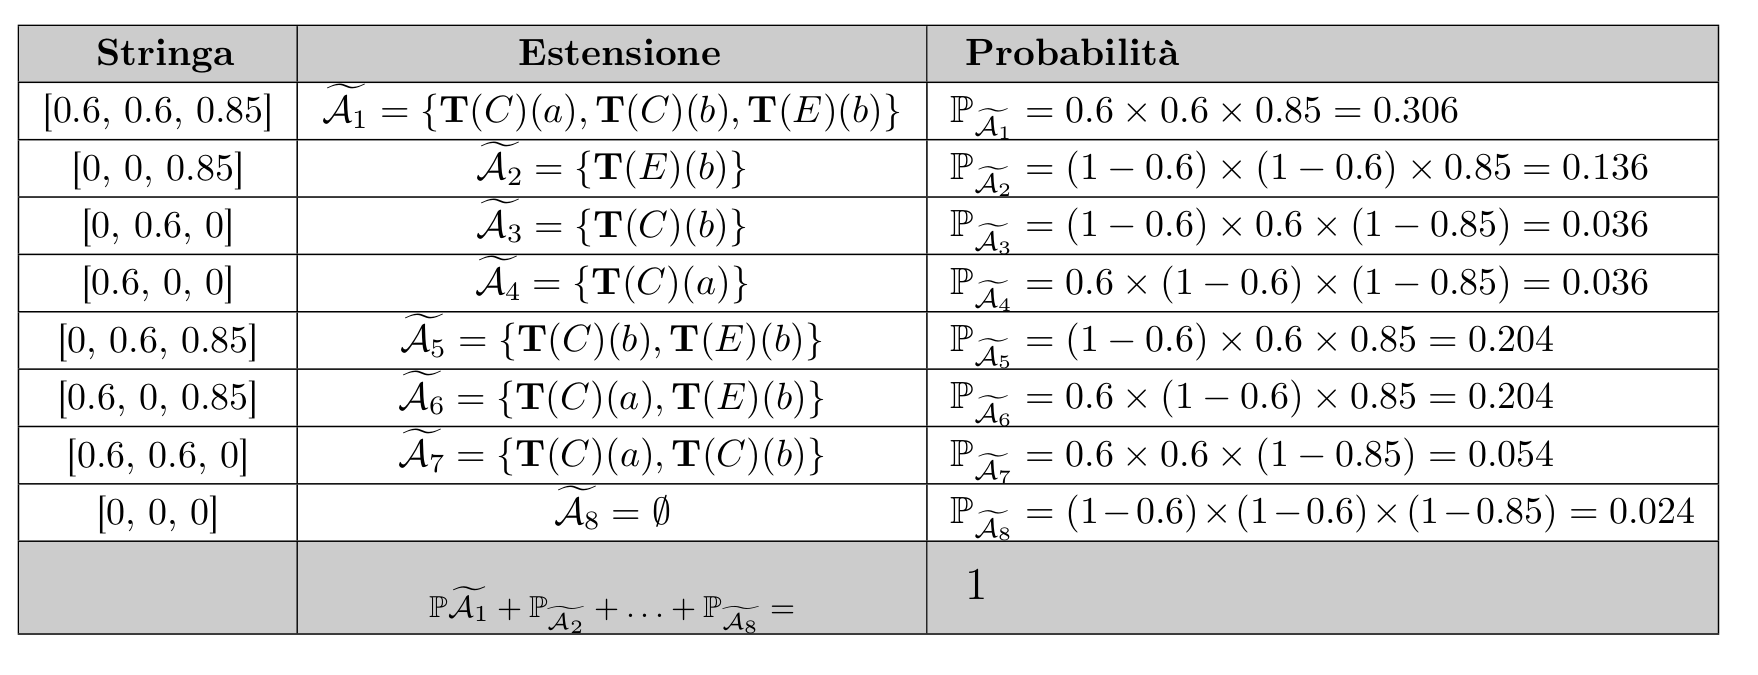
\includegraphics[width=\linewidth]{Estensione_Plausibile.png}
	\caption{Estensioni plausibili}
	\label{fig:estesioni}
	\centering
\end{figure}

\subsection{Dalla logica verso la "diagnosi"}
Descriviamo formalmente cosa si intenda per diagnosi in questo contesto particolare, aiutandoci con un esempio.
Data la seguente \textbf{KB} con \\ $ \textit{ABox} = \{MemoryLoss(Pietro)\} $ e \textit{TBox}:
\begin{itemize}
	\item $ Paranoia \sqsubseteq Depressed $
	\item $ \mathbf{T}(AlzheimerPatient) \sqsubseteq_{0.85} MemoryLoss $
	\item $ \mathbf{T}(AlzheimerPatient) \sqsubseteq_{0.65} Paranoia $
	\item $ \mathbf{T}(DiabetesPatient) \sqsubseteq_{0.90} Thirst $
	\item $ \mathbf{T}(DiabetesPatient) \sqsubseteq_{0.55} Depressed $
	\item $ \mathbf{T}(Depressed) \sqsubseteq_{0.80} Insomnia $
	\item $ \mathbf{T}(Depressed) \sqsubseteq_{0.70} Headache $
\end{itemize}

consideriamo un set $ \mathcal{V} $, espresso nella forma $ C(a) $, che rappresenta i sintomi e i segni nella forma:
\[ \mathcal{V} = \{ Paranoia(Pietro), Headache(Pietro) \} \]
sappiamo che  $ \mathcal{V} $ non è implicato dalla base di conoscenza, ma che $ \textbf{KB} \sqcup \mathcal{V} $ è \textit{consistente}.
Utilizzando la  logica $ \mathcal{ALC} + \mathbf{T}_{\mathbf{R}}^{\mathtt{P}} $ siamo interessati a trovare 
una diagnosi per i sintomi di $ Pietro $, cioè un insieme di \textit{asserzioni} $ D $ tali che $ \textbf{KB} \sqcup D \models \mathcal{V} $.\\
Seguendo l'esempio:
\begin{itemize}
	\item $ D_1 = \{AlzheimerPatient(Pietro)\} $ \textbf{segue logicamente}
	\item $ D_2 = \{Depressed(Pietro)\} $ \textbf{non segue logicamente}
	\item $ D_3 = \{AlzheimerPatient(Pietro), Depressed(Pietro)\} $ \textbf{segue logicamente}
\end{itemize}
che corrispondono a
\begin{itemize}
	\item \makebox[5,5cm]{$ \mathbf{T}(AlzheimerPatient)(Pietro) $\hfill} è implicato da $ \textbf{KB} \sqcup D_1 \land \textbf{KB} \sqcup D_3 $
	\item \makebox[5,5cm]{$ \mathbf{T}(Depressed)(Pietro) $ \hfill} è implicato solo in $ \textbf{KB} \sqcup D_3 $
	\item \makebox[5,5cm]{$ \mathbf{T}(DiabetesPatient)(Pietro) $ \hfill} non è implicato da nessuna \textbf{KB}
\end{itemize}
Possiamo ragionare sugli scenari, consideriamo, ad esempio, $ D_3 $ con 
\[ \mathfrak{Tip}_{\mathcal{A}} = {(Pietro,AlzheimerPatient), (Pietro,Depressed)} \] 
e con $ \mathcal{P_{A}} = [0.525,0.556] $ dove $ 0.525 = 0.85 \times 0.65 $ è la probabilità di equipaggiare
la proprietà tipica del concetto $ AlzheimerPatient $, discorso analogo per $ Depressed $.
Utilizzando quanto visto precedentemente si considerano le seguenti estensioni
\begin{itemize}
	\item \makebox[13.97cm]{$ \mathcal{\widetilde{A}}^3_1 = \{\mathbf{T}(AlzheimerPatient)(Pietro)\} $\hfill} 
		con $ \mathcal{P_{\widetilde{A}^\mathit{3_1}}} =  0.525 \times 0.463 = 0.243 $
	\item \makebox[13.97cm]{$ \mathcal{\widetilde{A}}^3_3 = \{\mathbf{T}(AlzheimerPatient)(Pietro), \mathbf{T}(Depressed)(Pietro)\} $ \hfill}
		con $ \mathcal{P_{\widetilde{A}^\mathit{3_3}}} = 0.556 \times 0.557 = 0.309  $
\end{itemize}
deduciamo, dunque, che:
\[ \textbf{KB} \sqcup D_i \models (\mathcal{ALC} + \mathbf{T}_{\mathbf{R}}^{\mathtt{P}}) ^{(0,1)} Paranoia(Pietro), Headache(Pietro) \]
con $ i = 1,3 $, vale a dire che tutte le asserzioni di cui sopra rappresentano una diagnosi per i sintomi $ \mathcal{V} $

E con questo concludiamo la trattazione dei fondamenti di logica.\\ 
Questa capitolo altro non è che un sunto, a tratti informale, della storia di questa branca matematica  
e non sostituisce certamente gli articoli e studi fatti nel corso degli anni, da figure molto più autorevoli,
della mia ma costituisce il corpo fondante di tutta la tesi.




